\documentclass[border=0.8ex,svgnames,tikz]{standalone}
\usepackage{amsmath,mathtools}
\usepackage{fontspec}
\setmainfont{Source Serif 4}
\setsansfont{Source Sans 3}
\setmonofont{Source Code Pro}
\usetikzlibrary{positioning,calc,fit,shapes,arrows.meta}
\usepackage{xparse}
\makeatletter
\NewDocumentCommand{\setbackground}{O{\nodewidth}O{\nodeheight}mmm}{%
  \begin{pgfinterruptboundingbox}
    \begin{scope}[local bounding box=bb@temp]
      \node[inner sep=0pt,fit=(#3)] {};
    \end{scope}
    \path($(bb@temp.north east)-(bb@temp.south west)$);
  \end{pgfinterruptboundingbox}
  \pgfgetlastxy{#1}{#2}
  \begin{scope}[
    every node/.style={
      minimum width=6.75em,
      minimum height=#4 * \nodeheight,
      fill=gray,
      fill opacity=0.4,
    },
    ]
    \node at ($(#3.north)!#5!(#3.south)$) {};
  \end{scope}
}
\makeatother
\begin{document}
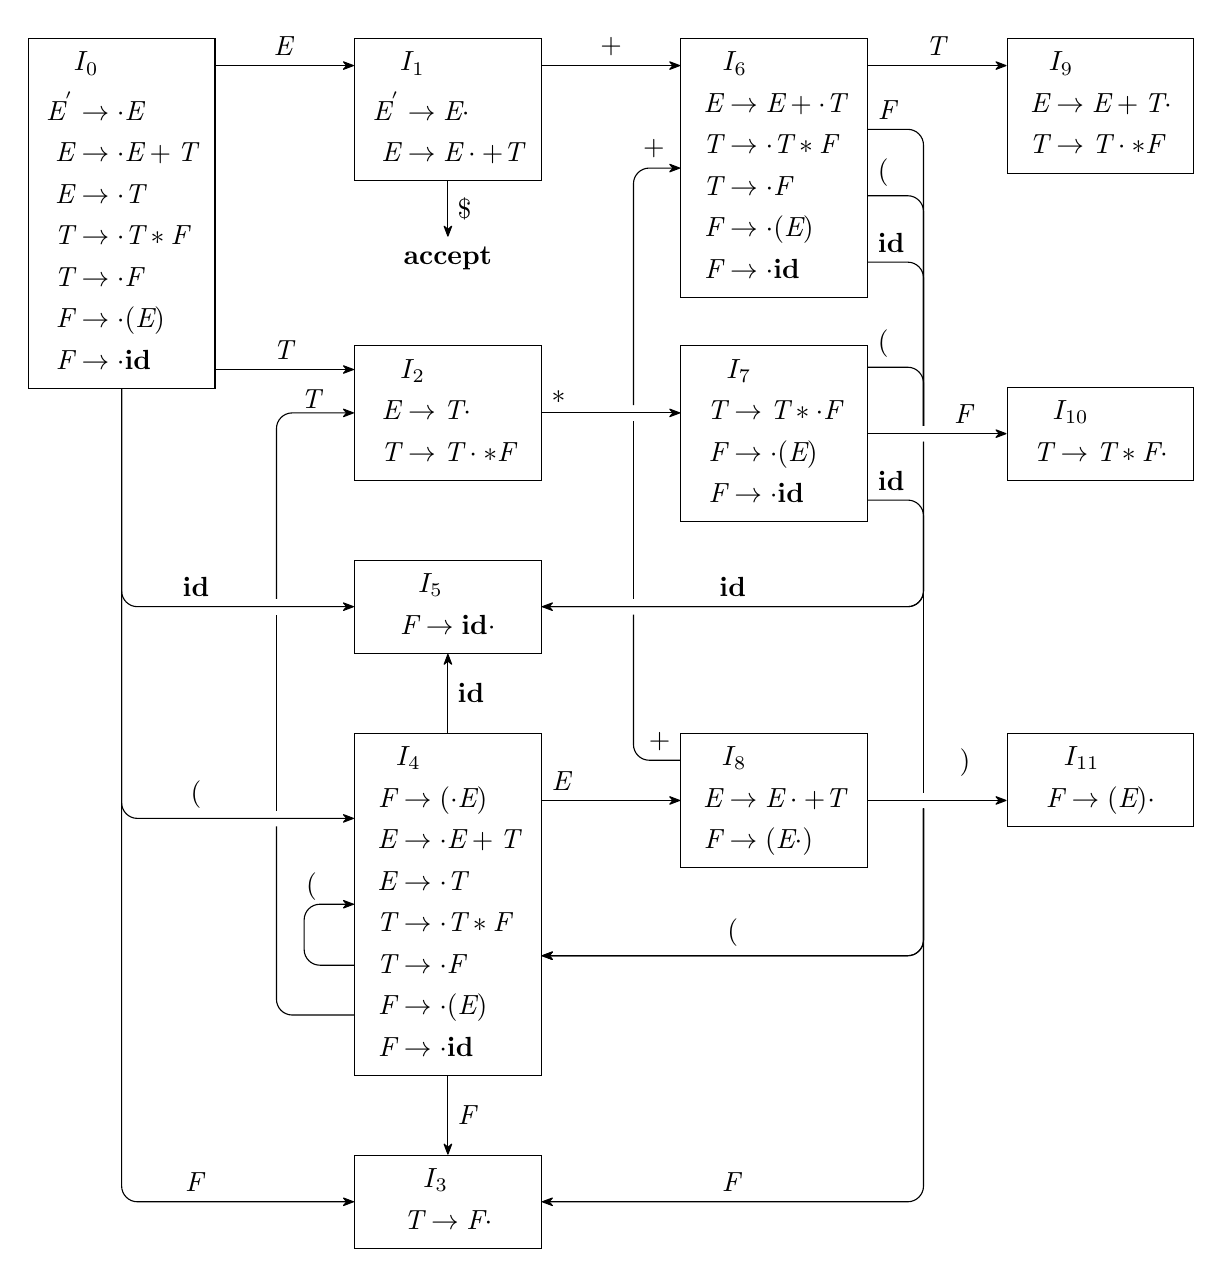
\begin{tikzpicture}
  \begin{scope}[
    every node/.style={
      rectangle,
      draw,
      minimum width=6.75em,
    },
    setanchor/.style={
      anchor=north west,
    },
  ]
    % I0
    \node (I0) at (0,0)
    {$\begin{aligned}
      & I_{0}\\
      \textit{E}^{'} &\rightarrow \cdot\textit{E}\\
      \textit{E} &\rightarrow \cdot\textit{E}+\textit{T}\\
      \textit{E} &\rightarrow \cdot\textit{T}\\
      \textit{T} &\rightarrow \cdot\textit{T}*\textit{F}\\
      \textit{T} &\rightarrow \cdot\textit{F}\\
      \textit{F} &\rightarrow \cdot(\textit{E})\\
      \textit{F} &\rightarrow \cdot\textbf{id}
    \end{aligned}$};

    % I1
    \node [right=5em of I0.north east,setanchor] (I1)
    {$\begin{aligned}
      & I_{1}\\
      \textit{E}^{'} &\rightarrow \textit{E}\cdot\\
      \textit{E} &\rightarrow \textit{E}\cdot+\textit{T}
    \end{aligned}$};

    % I6
    \node [right=5em of I1.north east,setanchor] (I6)
    {$\begin{aligned}
      & I_{6}\\
      \textit{E} &\rightarrow \textit{E}+\cdot\textit{T}\\
      \textit{T} &\rightarrow \cdot\textit{T}*\textit{F}\\
      \textit{T} &\rightarrow \cdot\textit{F}\\
      \textit{F} &\rightarrow \cdot(\textit{E})\\
      \textit{F} &\rightarrow \cdot\textbf{id}
    \end{aligned}$};

    % I9
    \node [right=5em of I6.north east,setanchor] (I9)
    {$\begin{aligned}
      & I_{9}\\
      \textit{E} &\rightarrow \textit{E}+\textit{T}\cdot\\
      \textit{T} &\rightarrow \textit{T}\cdot*\textit{F}
    \end{aligned}$};

    % I2
    \node [right=5em of $(I0.south east)!0.25!(I0.east)$,setanchor] (I2)
    {$\begin{aligned}
      & I_{2}\\
      \textit{E} &\rightarrow \textit{T}\cdot\\
      \textit{T} &\rightarrow \textit{T}\cdot*\textit{F}
    \end{aligned}$};

    % I7
    \node [right=5em of I2.north east,setanchor] (I7)
    {$\begin{aligned}
      & I_{7}\\
      \textit{T} &\rightarrow \textit{T}*\cdot\textit{F}\\
      \textit{F} &\rightarrow \cdot(\textit{E})\\
      \textit{F} &\rightarrow \cdot\textbf{id}
    \end{aligned}$};

    % I10
    \node [right=5em of I7] (I10)
    {$\begin{aligned}
      & I_{10}\\
      \textit{T} &\rightarrow \textit{T}*\textit{F}\cdot
    \end{aligned}$};

    % I5
    \node [below=of I2] (I5)
    {$\begin{aligned}
      & I_{5}\\
      \textit{F} &\rightarrow \textbf{id}\cdot
    \end{aligned}$};

    % I4
    \node [below=of I5] (I4)
    {$\begin{aligned}
      & I_{4}\\
      \textit{F} &\rightarrow (\cdot\textit{E})\\
      \textit{E} &\rightarrow \cdot\textit{E}+\textit{T}\\
      \textit{E} &\rightarrow \cdot\textit{T}\\
      \textit{T} &\rightarrow \cdot\textit{T}*\textit{F}\\
      \textit{T} &\rightarrow \cdot\textit{F}\\
      \textit{F} &\rightarrow \cdot(\textit{E})\\
      \textit{F} &\rightarrow \cdot\textbf{id}
    \end{aligned}$};

    % I8
    \node [right=5em of I4.north east,setanchor] (I8)
    {$\begin{aligned}
      & I_{8}\\
      \textit{E} &\rightarrow \textit{E}\cdot+\textit{T}\\
      \textit{F} &\rightarrow (\textit{E}\cdot)
    \end{aligned}$};

    % I11
    \node [right=5em of I8.north east,setanchor] (I11)
    {$\begin{aligned}
      & I_{11}\\
      \textit{F} &\rightarrow (\textit{E})\cdot
    \end{aligned}$};

    % I3
    \node [below=of I4] (I3)
    {$\begin{aligned}
      & I_{3}\\
      \textit{T} &\rightarrow \textit{F}\cdot
    \end{aligned}$};
  \end{scope}
  \setbackground{I0}{0.74}{0.63}
  \setbackground{I4}{0.74}{0.63}
  \setbackground{I6}{0.66}{0.67}
  \setbackground{I7}{0.52}{0.74}
  \begin{scope}[
    myarrow/.style={
      ->,
      rounded corners=2mm,
      >=Stealth[round],
      % very thick,
    },
    ]
    % Path I0
    \draw [myarrow] (I0.north east) ++(0,-1.em) -- node [above] {\textit{E}} ++(5em,0);
    \draw [myarrow] (I0.south east) ++(0,0.7em) -- node [above] {\textit{T}} ++(5em,0);
    \draw [myarrow] (I0.south) |- (I5.west);
    \draw [myarrow] (I0.south) |- ($(I4.west)!0.5!(I4.north west)$) coordinate (oI0iI4);
    \draw [myarrow] (I0.south) |- (I3.west);
    \draw (oI0iI4) ++(-2.8em,-0.1) coordinate (I4interrupt1);
    \draw (oI0iI4) ++(-2.8em,+0.1) coordinate (I4interrupt2);
    \draw (I5.west) ++(-2.8em,-0.1) coordinate (I5interrupt1);
    \draw (I5.west) ++(-2.8em,+0.1) coordinate (I5interrupt2);
    \node [above] at ($(I0.south |- I5.west)!0.32!(I5.west)$) {\textbf{id}};
    \node [above] at ($(I0.south |- oI0iI4)!0.32!(oI0iI4)$) {\((\)};
    \node [above] at ($(I0.south |- I3.west)!0.32!(I3.west)$) {\textit{F}};

    % Path I1
    \draw [myarrow] (I1.north east) ++(0,-1em) -- node [above] {\(+\)} ++(5em,0);
    \draw [myarrow] (I1.south) -- node [right] {\(\$\)} ++(0,-2em) node[below]
    {\textbf{accept}};

    % Path I2
    \draw [myarrow] (I2.east) node [above right] {\(*\)} -- ++(5em,0);

    % Path I4
    \draw [myarrow,-] (I4.south west) ++(0,2.2em) -- ++(-2.8em,0) -- (I4interrupt1);
    \draw [myarrow,-] (I4interrupt2) -- (I5interrupt1);
    \draw [myarrow] (I5interrupt2) |- (I2.west);
    \draw [myarrow] (I4) -- node [right] {\textit{F}} (I3);
    \draw [myarrow] (I4.south west) ++ (0,4em) -- ++(-1.8em,0) |- (I4.west);
    \draw [myarrow] (I4) -- node [right] {\textbf{id}} (I5);
    \draw [myarrow] (I8.west) ++(-5em,0) node [above right] {\textit{E}} -- (I8);
    \node [label=left:$\textit{T}$,below right=-1.2em] at (I2.west) {};
    \node [label=left:$($,below right=-1.4em] at (I4.west) {};

    % Interrupt
    \draw (I2.east) ++(3.31em,-0.1) coordinate (I2interrupt1);
    \draw (I2.east) ++(3.31em,+0.1) coordinate (I2interrupt2);
    \draw (I5.east) ++(3.31em,-0.1) coordinate (I5interrupt3);
    \draw (I5.east) ++(3.31em,+0.1) coordinate (I5interrupt4);
    \draw (I7.east) ++(2em,-0.1) coordinate (I7interrupt1);
    \draw (I7.east) ++(2em,+0.1) coordinate (I7interrupt2);
    \draw (I8.east) ++(2em,-0.1) coordinate (I8interrupt1);
    \draw (I8.east) ++(2em,+0.1) coordinate (I8interrupt2);

    % Path I6
    \draw [myarrow,-] (I6.east) ++(0,1.4em) coordinate (oI6iI3start) -- ++(2em,0) --
    (I7interrupt2);
    \draw [myarrow,-] (I7interrupt1) -- (I8interrupt2);
    \draw [myarrow] (I8interrupt1) |- coordinate (oI6iI3mid) (I3);
    \draw [myarrow,-] (I6.east) ++(0,-1em) coordinate (oI6iI4start) -- ++(2em,0) --
    (I7interrupt2);
    \draw [myarrow,-] (I7interrupt1) -- (I8interrupt2);
    \draw [myarrow] (I8interrupt1) |- coordinate (oI6iI4mid)
    ($(I4.east)!0.3!(I4.south east)$) coordinate (oI6iI4);
    \draw [myarrow,-] (I6.east) ++(0,-3.4em) coordinate (oI6iI5start) --
    ++(2em,0) -- (I7interrupt2);
    \draw [myarrow,-] (I7interrupt1) |- coordinate (oI6iI5mid) (I5);
    \draw [myarrow] (I6.north east) ++(0,-1em) -- node [above] {\textit{T}}
    ++(5em,0);
    \node [above] at ($(oI6iI3mid)!0.5!(I3.east)$) {\textit{F}};
    \node [label=above right:$\textit{F}$,below left] at (oI6iI3start) {};
    \node [above] at ($(oI6iI4mid)!0.5!(oI6iI4)$) {\((\)};
    \node [label=above right:$($,below left] at (oI6iI4start) {};
    \node [above] at ($(oI6iI5mid)!0.5!(I5.east)$) {\textbf{id}};
    \node [label=above right:$\textbf{id}$,below left] at (oI6iI5start) {};

    % Path I7
    \draw [myarrow,-] (I7.east) ++(0,2.4em) coordinate (oI7iI4start) -- ++(2em,0) --
    (I7interrupt2);
    \draw [myarrow,-] (I7interrupt1) -- (I8interrupt2);
    \draw [myarrow] (I8interrupt1) |-
    (oI6iI4);
    \draw [myarrow] (I7.east) ++(0,-2.4em) coordinate (oI7iI5start) -- ++(2em,0) |-
    (I5);
    \draw [myarrow] (I7.east) -- ++(5em,0);
    \node [label=above right:$($,below left] at (oI7iI4start) {};
    \node [label=above right:$\textbf{id}$,below left] at (oI7iI5start) {};
    \node [above] at ($(I7.east)!.7!(I10.west)$) {\textit{F}};

    % Path I8
    \draw [myarrow] (I8.east) -- ++(5em,0);
    \draw [myarrow,-] (I8.north west) ++(0,-1em) node [above left] {\(+\)} --
    ++(-1.69em,0) -- (I5interrupt3);
    \draw [myarrow,-] (I5interrupt4) -- (I2interrupt1);
    \draw [myarrow] (I2interrupt2) |- node [label=above right:$+$,below left] {} (I6);
    \node [above] at ($(I8.east)!.7!(I11.west)$) {\()\)};
  \end{scope}
\end{tikzpicture}
\end{document}
